%%%%%%%%%%%%%%%%%%%%%%%%%%%%%%%%%%%%%%%%%
% baposter Landscape Poster
% LaTeX Template
% Version 1.0 (11/06/13)
%
% baposter Class Created by:
% Brian Amberg (baposter@brian-amberg.de)
%
% This template has been downloaded from:
% http://www.LaTeXTemplates.com
%
% License:
% CC BY-NC-SA 3.0 (http://creativecommons.org/licenses/by-nc-sa/3.0/)
%
%%%%%%%%%%%%%%%%%%%%%%%%%%%%%%%%%%%%%%%%%

%----------------------------------------------------------------------------------------
%	PACKAGES AND OTHER DOCUMENT CONFIGURATIONS
%----------------------------------------------------------------------------------------

\documentclass[landscape,a0paper,fontscale=0.285]{baposter} % Adjust the font scale/size here

\usepackage{graphicx} % Required for including images
\graphicspath{{figures/}} % Directory in which figures are stored

\usepackage{amsmath} % For typesetting math
\usepackage{amssymb} % Adds new symbols to be used in math mode

\usepackage{booktabs} % Top and bottom rules for tables
\usepackage{enumitem} % Used to reduce itemize/enumerate spacing
\usepackage{palatino} % Use the Palatino font
\usepackage[font=small,labelfont=bf]{caption} % Required for specifying captions to tables and figures

\usepackage{multicol} % Required for multiple columns
\setlength{\columnsep}{1.5em} % Slightly increase the space between columns
\setlength{\columnseprule}{0mm} % No horizontal rule between columns

\usepackage{tikz} % Required for flow chart
\usetikzlibrary{shapes,arrows} % Tikz libraries required for the flow chart in the template

\newcommand{\compresslist}{ % Define a command to reduce spacing within itemize/enumerate environments, this is used right after \begin{itemize} or \begin{enumerate}
\setlength{\itemsep}{1pt}
\setlength{\parskip}{0pt}
\setlength{\parsep}{0pt}
}

\definecolor{lightblue}{rgb}{0.145,0.6666,1} % Defines the color used for content box headers

\begin{document}

\begin{poster}
{
headerborder=closed, % Adds a border around the header of content boxes
colspacing=1em, % Column spacing
bgColorOne=white, % Background color for the gradient on the left side of the poster
bgColorTwo=white, % Background color for the gradient on the right side of the poster
borderColor=lightblue, % Border color
headerColorOne=black, % Background color for the header in the content boxes (left side)
headerColorTwo=lightblue, % Background color for the header in the content boxes (right side)
headerFontColor=white, % Text color for the header text in the content boxes
boxColorOne=white, % Background color of the content boxes
textborder=roundedleft, % Format of the border around content boxes, can be: none, bars, coils, triangles, rectangle, rounded, roundedsmall, roundedright or faded
eyecatcher=true, % Set to false for ignoring the left logo in the title and move the title left
headerheight=0.1\textheight, % Height of the header
headershape=roundedright, % Specify the rounded corner in the content box headers, can be: rectangle, small-rounded, roundedright, roundedleft or rounded
headerfont=\Large\bf\textsc, % Large, bold and sans serif font in the headers of content boxes
%textfont={\setlength{\parindent}{1.5em}}, % Uncomment for paragraph indentation
linewidth=2pt % Width of the border lines around content boxes
}
%----------------------------------------------------------------------------------------
%	TITLE SECTION
%----------------------------------------------------------------------------------------
%
{
\includegraphics[height=4em]{logo.png}} % First university/lab logo on the left
{\bf\textsc{Deep Neural Network Classifier of Handwritten digits}\vspace{0.5em}} % Poster title
{\textsc{\{ Mohammad Reza Sanatkar, Mengke Lian \} \hspace{12pt} Duke University - ECE Department}} % Author names and institution
{
\includegraphics[height=4em]{logo.png}} % Second university/lab logo on the right

%----------------------------------------------------------------------------------------
%	OBJECTIVES
%----------------------------------------------------------------------------------------

\headerbox{Objectives}{name=objectives,column=0,row=0}{

This course project aims at dealing with hand writing recognition task.
Deep neural networks have garnered a lot of attention in the field of machine learning in the recent years. In this project, we implement a multi-layer neural networks to perform the task of handwritten digits. Our project can be divided in the following main steps: 

\begin{itemize}
\item   Implementation of a general class of multi-layer neural networks in C++.
\item   Implementation of feed-forward and back-propagation algorithm to train such networks as discriminative classifiers.
\item   Implementation of learning algorithm for RBM to train neural networks as generative classifiers.
\end{itemize}

\vspace{0.3em} % When there are two boxes, some whitespace may need to be added if the one on the right has more content
}

%----------------------------------------------------------------------------------------
%	INTRODUCTION
%----------------------------------------------------------------------------------------

\headerbox{Introduction}{name=introduction,column=1,row=0,bottomaligned=objectives}{

Multi-layer neural networks represent the consistent effort of human beings to mimic the brain. Below, you see the neural networks which is used in this project. This network consists of three hidden layers.
\begin{center}
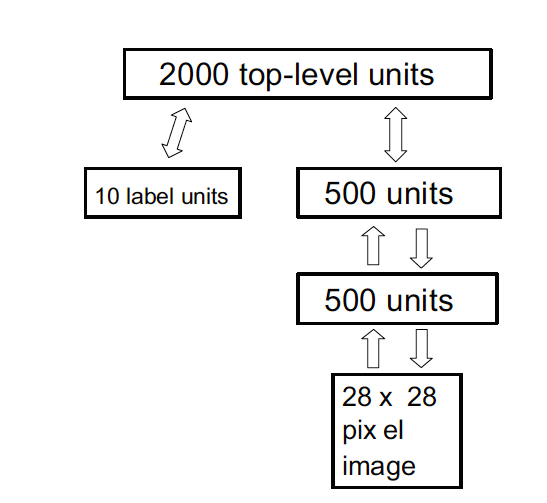
\includegraphics[width=0.6\linewidth]{DNN.png}
\captionof{figure}{Neural Network implemented as a classifier of handwritten digits [1]}
\end{center}

}
%----------------------------------------------------------------------------------------
%	RESULTS 1
%----------------------------------------------------------------------------------------

\headerbox{Restricted Boltzmann Machine (RBM)}{name=results,column=2,span=2,row=0}{

\begin{multicols}{2}
Deep belief networks outperform the traditional neural networks  because of taking benefits from RBMs. What is a RBM? RBM is a bipartite undirected inference graph which is used to learn a multivariate joint distribution satisfying the conditional independence imposed by the bipartite structure of the graph. In deep neural networks, every pair of successive layers is considered as a RBM. The first and most important step of training a deep neural network is to train these RBMs.\\
\indent First, we train the RBM corresponding to the input layer and the first hidden layer. After learning the generative model for the first RBM, we use this set of learned weights to generate inputs for the second RBM. Having inputs for the second RBM, the set of weights of edges entering the nodes in the second hidden layer are learnt. These steps are repeated for all the other RBMS too.\\


\end{multicols}

%------------------------------------------------

\begin{multicols}{2}
\vspace{1em}
How to learn a RBM in a reasonable time : Contrastive Divergence Learning Procedure\\
\begin{equation}
\Delta w_{ij} = \epsilon (<v_{i}h_{j}>^{0} - <v_{i}h_{j}^{1})\nonumber
\end{equation}
\begin{itemize}
\item Start with available data on the visible units
\item Compute the hidden nodes in parallel
\item Compute the visible units (Reconstruction)
\item Update the hidden nodes again
\end{itemize}

\begin{center}
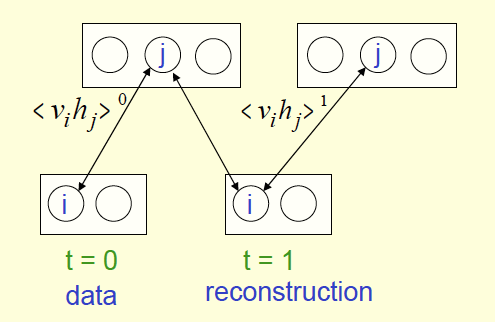
\includegraphics[width=0.8\linewidth]{CDLP.png}
\captionof{figure}{Contrastive Divergence Learning[1] }
\end{center}

\end{multicols}
}



%----------------------------------------------------------------------------------------
%	MATERIALS AND METHODS
%----------------------------------------------------------------------------------------

\headerbox{MNIST Database}{name=method,column=0,below=objectives}{ % This block's bottom aligns with the bottom of the conclusion block

The MNIST database of handwritten digits contains a training set of 60,000 examples, and a test set of 10,000 examples.
\vspace{5pt}

Each image is transformed from bilevel (black and white) image from NIST database by renormalizing to fit in a $20\times20$ pixel box while preserving aspect ration, which result into a $20\times20$ grey-scaled image.
And then this $20\times20$ grey-scaled image is centered in a $28\times28$ image by computing the center of mass of the pixels, and translating the image so as to position this point at the center of the $28\times28$ field.
\vspace{5pt}
The dataset consists of:
\begin{itemize}
\item   60000 training images of handwritten digits as well as their labels
\item   10000 images of handwritten digits as test data
\end{itemize}
}



%----------------------------------------------------------------------------------------
%	CONCLUSION
%----------------------------------------------------------------------------------------

\headerbox{Conclusion}{name=conclusion,column=2,span=2,row=0,below=results, bottomaligned=method}{
\begin{multicols}{2}
Neural networks became popular in the community of compute scientists after derivation of back-propagation by Hinton in 1985. However,  many researchers abandoned it because of emergence of SVM in 1990's. SVM worked better than trained neural networks by back-propagation. In 2002, Hinton came up with a fast method to train RBM neural networks which outperformed SVM classifiers. \\
We need to note that the significant increase in computational power of the computers in the recent years had a key role to make RBM neural networks practical. Training a deep neural networks as a generative classifier needs a huge amount of computations in parallel. Below, you can see the comparison between the RBM neural network and the other methods for handwritten digits recognition of MNIST dataset. the RBM deep neural network works better than other methods. 


%------------------------------------------------

\begin{itemize}\compresslist
\item Generative model based on RBMs                 1.25\%
\item Support Vector Machine (Decoste et. al.)	     1.4\%	
\item Backprop with 1000 hiddens (Platt)                1.6\%
\item Backprop with 500 -->300 hiddens                 1.6\%
\item K-Nearest Neighbor                                        3.3\%
\end{itemize}

\end{multicols}
}

%----------------------------------------------------------------------------------------
%	RESULTS 2
%----------------------------------------------------------------------------------------

\headerbox{Back-Propagation}{name=results2,column=1,below=objectives, bottomaligned=method}{ % This block's bottom aligns with the bottom of the conclusion block

Back-propagation calculates the gradient of a loss function with respects to all the weights in the network.
The gradient is fed to the optimization method which in turn uses it to update the weights, in an attempt to minimize the loss function.
\vspace{5pt}

Denote the loss function as $J$, the basic iteration step in gradient descent is given by: 
\[ \Delta w = \ell \nabla J, \quad \Delta w_i = \ell \frac{\partial J}{\partial w_i} \]
%The back-propagation algorithm consists of applying the chain rule to compute these partial derivatives.
%\vspace{5pt}

For training images $ \{(X_i,y_i)\}_{i=1}^N$, each time we use $X_i$ as input and get the output $\hat{y}_i$ by feed-forward.
Since we know the $y_i$, once $\hat{y}_i$ is known then $J$ is determined and back-propagation is applied to update the weights.
%The training process stops after all the training images are used for the procedure above.
}
%----------------------------------------------------------------------------------------


%----------------------------------------------------------------------------------------
%	REFERENCES
%----------------------------------------------------------------------------------------

\headerbox{References}{name=references,column=0,above=bottom,below=method}{

\renewcommand{\section}[2]{\vskip 0.05em} % Get rid of the default "References" section title
\nocite{*} % Insert publications even if they are not cited in the poster
\small{ % Reduce the font size in this block
\bibliographystyle{unsrt}
\bibliography{sample} % Use sample.bib as the bibliography file
}}




%----------------------------------------------------------------------------------------
%	FUTURE RESEARCH
%----------------------------------------------------------------------------------------

\headerbox{Future Research}{name=futureresearch,column=1,span=2,aligned=references, above=bottom}{ % This block is as tall as the references block

%\begin{multicols}{2}
%All the major technology companies adopted deep neural networks to improve the performance of their products in the recent years. 
Even though employing multi-layer neural networks have improved the accuracy of object detection systems, the success rate of such systems is about 50 percent. This gives rise to the idea of a new class of neural networks with more similar structure to brain.
%\end{multicols}
}

%----------------------------------------------------------------------------------------
%	CONTACT INFORMATION
%----------------------------------------------------------------------------------------

\headerbox{Contact Information}{name=contact,column=3,aligned=references, above=bottom}{ % This block is as tall as the references block

\begin{description}\compresslist
\item[Email] reza.sanatkar@duke.edu
\item[Email] mengke.lian@duke.edu
\end{description}
}


\end{poster}

\end{document}
